\documentclass[10pt]{beamer}

\usetheme[progressbar=frametitle]{metropolis}

% Correcciones para Miktex en Windows:

% map defaulf alertblock to oldalertblock
\let\oldalertblock\alertblock{}
\let\endoldalertblock\endalertblock{}

% change alertblock by adding smallskip
\renewenvironment{alertblock}[1]
    {\begin{oldalertblock}{#1}
        \smallskip
    }
    {
    \end{oldalertblock}
    }

% map defaulf block to oldblock
\let\oldblock\block{}
\let\endoldblock\endblock{}

% change block by adding smallskip
\renewenvironment{block}[1]
    {\begin{oldblock}{#1}
        \smallskip
    }
    {
    \end{oldblock}
    }

\usepackage{appendixnumberbeamer}
\usepackage{ragged2e}
\usepackage[spanish]{babel}       %Paquete del lenguaje de caracteres en español.
\selectlanguage{spanish}        %Seleccion de lenguaje del documento.
\usepackage{fontenc}          % (este comando parte bien las palabras en castellano)
\usepackage{wrapfig}
\usepackage{amsmath, amssymb}

% \usepackage{sansmathaccent}
% \pdfmapfile{+sansmathaccent.map}
% \usepackage[sfdefault]{FiraSans}

%\usepackage{enumitem}          %paquete para listas de variacion para listas.
\usepackage{xparse}         %Paquete recomendado por "physics"
\usepackage{physics}          %Paquete de herramientas de física.
\usepackage{qcircuit}         %Paquete de circuitos cuánticos.
\usepackage{booktabs}
\usepackage[scale=2]{ccicons}

\usepackage{pgfplots}
\usepgfplotslibrary{dateplot}

\usepackage{xspace}
\newcommand{\themename}{\textbf{\textsc{metropolis}}\xspace}
\newcommand{\K}[1]{$\ket{#1}$}
\title{Redes de comunicación cuántica a grandes escalas}
\date{\today}
\date{\textcolor{black}{noviembre 2022} }
\author{\textcolor{black}{Marco Méndez y Alfredo Villegas}}
\institute{\textcolor{black}{Universidad Simón Bolívar}}
\titlegraphic{\hfill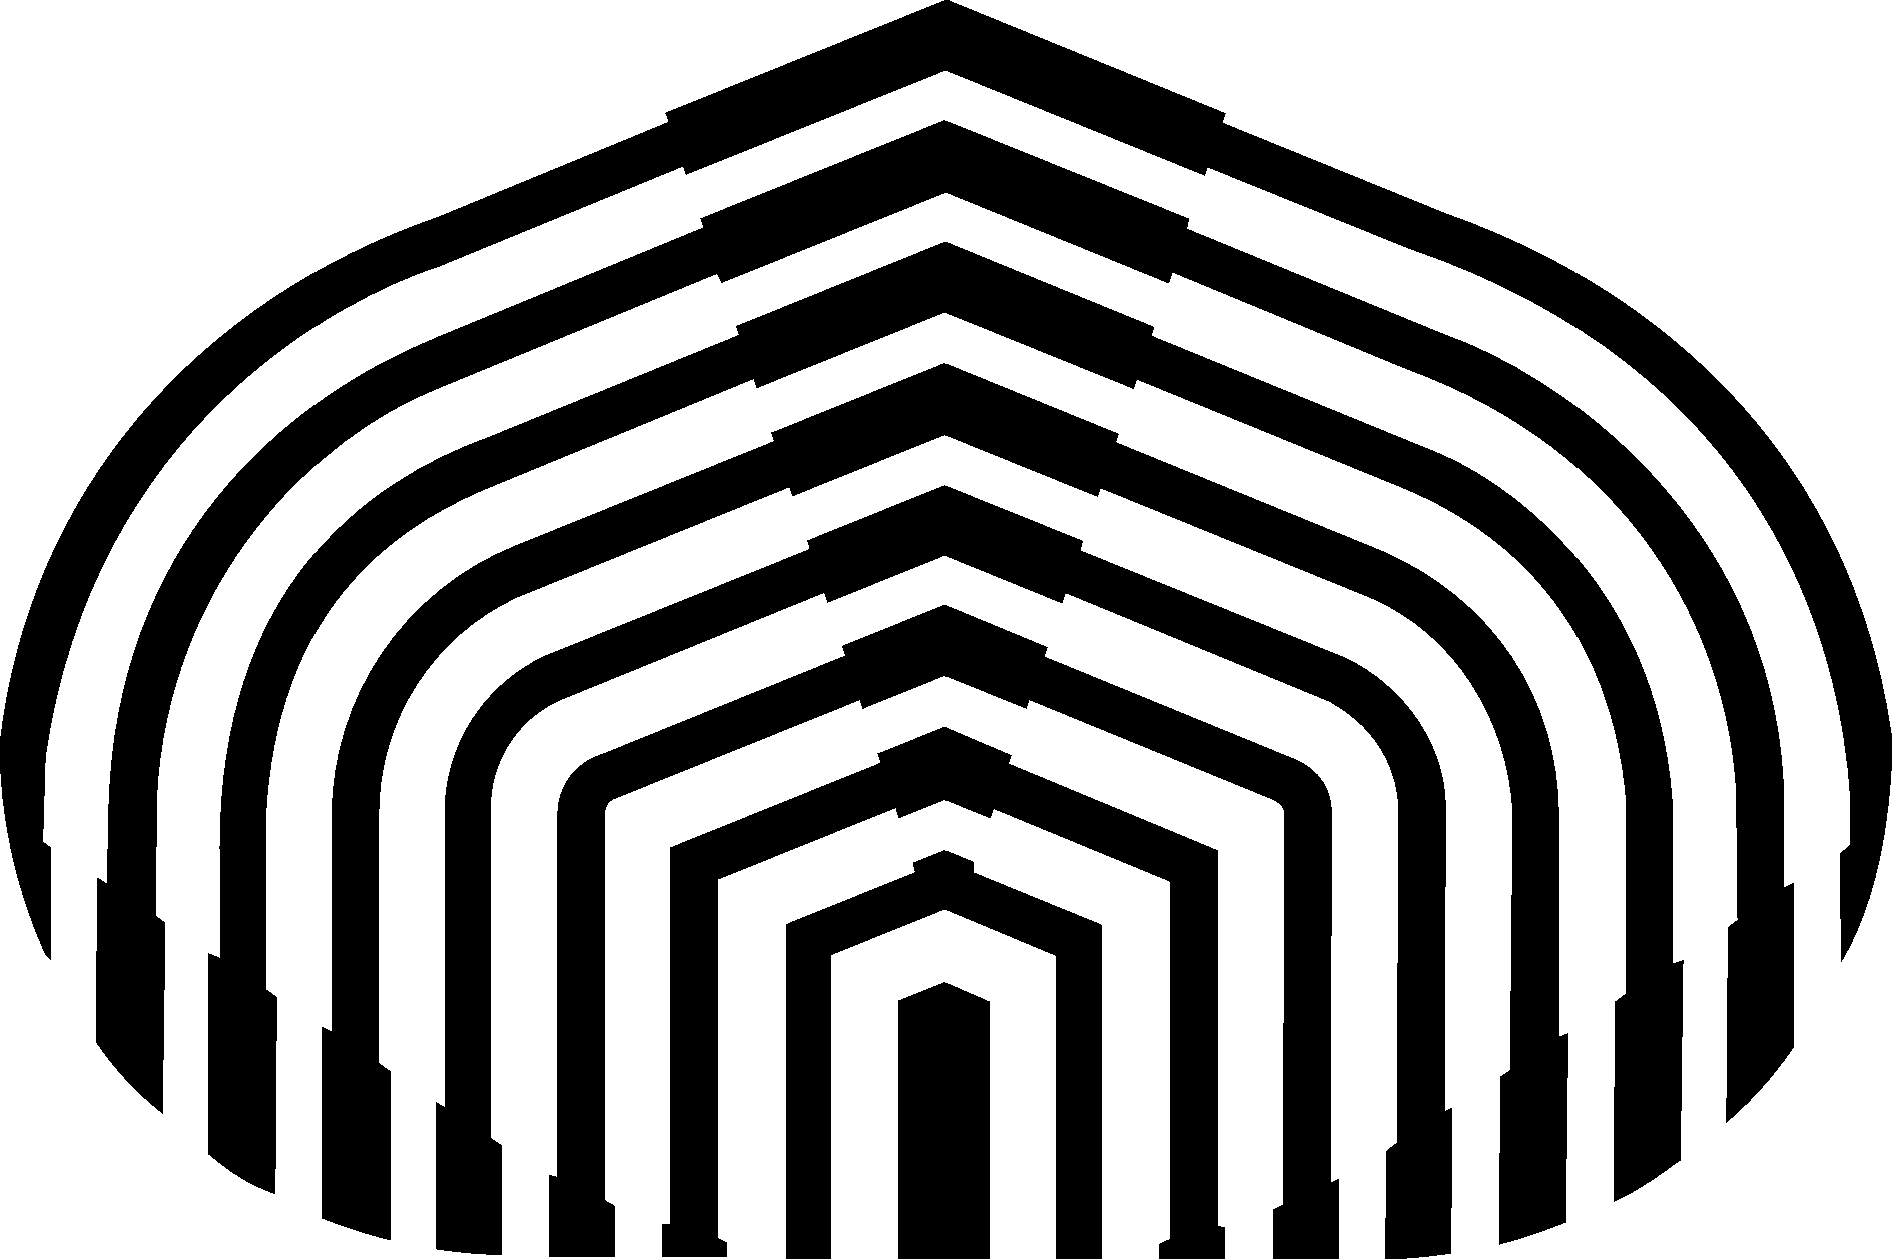
\includegraphics[height=1.0cm]{Cebollita_usb.png}}
\setbeamercolor{normal text}{fg=black,bg=white}
\definecolor{miscolorines}{HTML}{0B6DD5}
\setbeamercolor{alerted text}{fg=miscolorines,bg=white}

\begin{document}

\maketitle

\section{Resumen}
\begin{frame}{Resumen}
  \justifying{
    La codificación de redes cuánticas de gran escala, en inglés: Large-scale quantum network coding (LQNC) Es un método pensado para distribuir qubits entrelazados por redes de comunicación cuántica de grandes escalas que soportan la teleportación y la distribución de claves cuánticas. \par El proceso consta de un procedimiento de codificación para distribuir pares entrelazados de qubits entre los pares de usuarios emisor-receptor conectados por una ruta troncal de N saltos.  El tipo de red propuesta se conoce como red mariposa. El sistema propuesto es entonces comparado con  los sistemas basados en el entrelazamiento de intercambio para resaltar los beneficios.}
\end{frame}
%%%%%%%%%%%%%%%%%%%%%%%%%%%%%%%%%%%%%%%%%%%%%%%

\begin{frame}{Esquema}
  \setbeamertemplate{section in toc}[sections numbered]
  \tableofcontents[hideallsubsections]
\end{frame}
%%%%%%%%%%%%%%%%%%%%%%%%%%%%%%%%%%%%%%%%%%%%%%%%

\section{Codificación de redes cuánticas}
%%------------------------------------%%
\begin{frame}{Redes de comunicación cuántica}
  Las \textbf{redes de comunicación cuántica} abarcan el caso en el que se tienen más de dos nodos, estableciendo así topologías diversas en donde se tiene como objetivo transmitir qubits desde usuarios fuentes hacia usuarios objetivos vía teleportación.
  \begin{figure}
    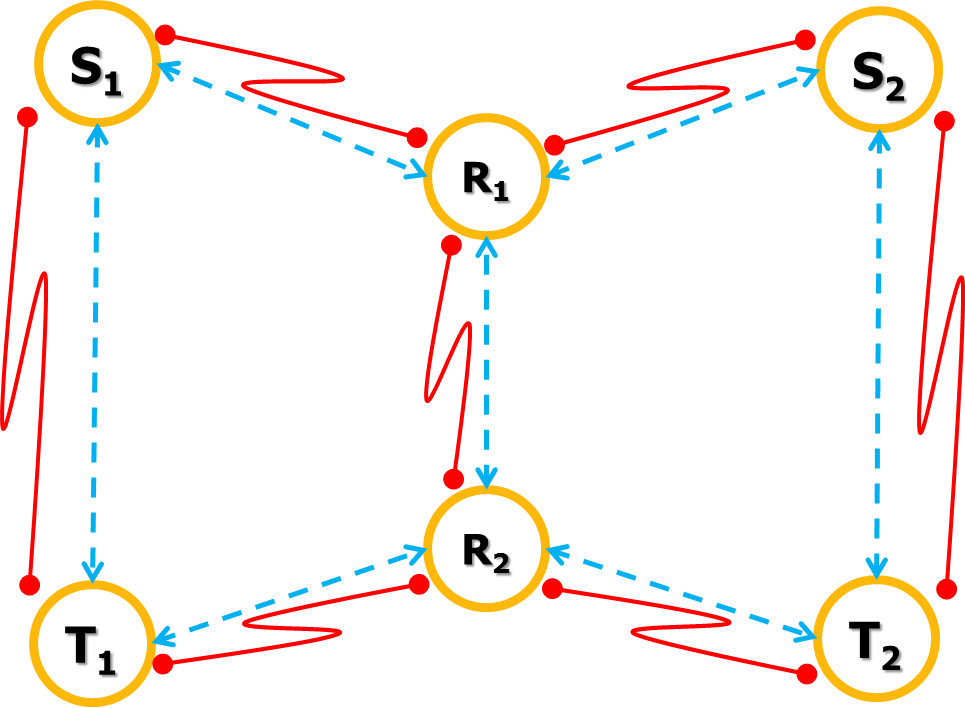
\includegraphics[width=0.5\textwidth]{butterflyquantum.png}
    \caption{Ejemplo de red cuántica tipo mariposa.}
    \label{fig:butterfly1}
  \end{figure}%
\end{frame}
%%------------------------------------%%
\begin{frame}{Codificación de redes cuánticas}
  El método más eficiente para establecer entrelazamiento entre usuarios de una red separados por nodos repetidores es la \alert{codificación de redes cuánticas}. \par
  El método consiste en realizar operaciones no unitarias sobre los estados entrelazados de los nodos con el fin de obtener un entrelazamiento entre los nodos deseados.
  \begin{figure}
    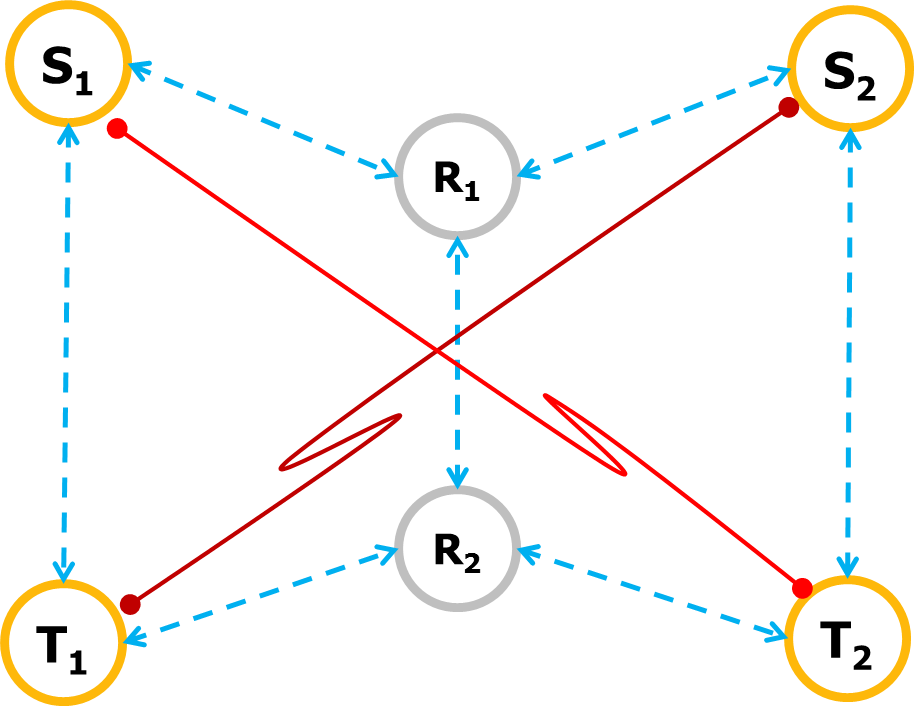
\includegraphics[width=0.4\textwidth]{butterflycoded.png}
    \caption{Red cuántica luego de la codificación}
  \end{figure}
\end{frame}
%%------------------------------------%%
\begin{frame}{Operaciones no unitarias de la codificación de redes}
  Las operaciones no unitarias de codificación están basadas en \alert{circuitos cuánticos} compuestos por operaciones unitarias y de medida. Estas son:
  \begin{itemize}
    \item Connect \item Removal \item Fanout \item Add \item RemAdd
  \end{itemize}
  Estas operaciones son \textit{no unitarias}, debido a que no preservan la cantidad de particiones del estado de entrada y de salida. \par
  Dado que estas operaciones se realizan en redes cuánticas es \textbf{importante} observar que las particiones de los estados entrelazados se encuentran físicamente en \textbf{nodos distantes}. \par
\end{frame}
%%------------------------------------%%
\begin{frame}{Operación Connect}
  Los estados $\ket{AB}$ y $\ket{CD}$ son estados máximamente entrelazados, como por ejemplo los estados de Bell, el circuito transforma estos dos estados y los \textbf{conecta} descartando una de las particiones para así tener un estado entrelazado de tres particiones a la salida.
  \vspace{-2em}
  \begin{figure}
    \[
      \Qcircuit @C=2em @R=0em @!R{
      \lstick{\ket{A}} & \ctrl{3} & \qw & \qw & \qw \\
      \lstick{\ket{B}} & \qw  & \qw & \qw & \qw \\
      &  & & & \\
      \lstick{\ket{C}} & \targ & \measure{M_Z} & \cctrl{1} & \\
      \lstick{\ket{D}} & \qw & \qw & \gate{X} & \qw
      } \]
    \caption{Diagrama de circuito cuántico de la Operación Connect }
  \end{figure}
  \vspace{-0.5em}
  El estado a la salida es un estado tripartito máximamente entrelazado. Por ejemplo el estado GHZ.
  \begin{align*}
  \ket{\psi_{out}} = 
  \frac{1}{\sqrt{2}} (\ket{000}_{ABD} + \ket{111}_{ABD}) 
  \end{align*}
\end{frame}
%%------------------------------------%%
\begin{frame}{Operación Removal}
  \begin{block}{}
    La operación está concebida para \textbf{remover} un qubit de un estado entrelazado, aplicando la compuerta Hadamard y luego midiendo ese qubit en la base ``$+$'' (también llamada base $Z$), el resultado de esa medida controla la compuerta $Z$ en la partición ``B'', de esta forma se evita una posible pérdida de información.
  \end{block}
  \begin{figure} \vspace{-0.5cm}
    \[
      \Qcircuit @C=2em @R=0em @!R{
      \lstick{\ket{A}} & \gate{H} & \measure{M_Z} & \cctrl{1} & \\
      \lstick{\ket{B}} & \qw & \qw &  \gate{Z} & \qw \\
      \lstick{\ket{C}} & \qw & \qw & \qw & \qw \\
      }\]
    \caption{Diagrama de circuito cuántico de la Operación Removal}
  \end{figure}
\end{frame}
%%------------------------------------%%
\begin{frame}{Operación Add}
  \begin{block}{}
    Esta operación es muy similar a Connect, la diferencia radica en la compuerta CNOT adicional con otro par EPR. 
  \end{block}
  \begin{figure}
    \[
      \Qcircuit @C=2em @R=0em @!R{
      \lstick{\ket{A}} & \qw & \qw & \qw & \qw & \qw \\
      \lstick{\ket{B}} & \ctrl{5} & \qw & \qw & \qw & \qw  \\
      &  & & & \\
      \lstick{\ket{C}} & \qw & \qw & \qw & \qw & \qw \\
      \lstick{\ket{D}} & \qw & \ctrl{2} & \qw & \qw & \qw \\
      &  & & & \\
      \lstick{\ket{E}} & \targ & \targ & \measure{M_Z} & \cctrl{1}  \\
      \lstick{\ket{F}} & \qw & \qw & \qw & \gate{X} & \qw \\
      }\]
    \caption{Diagrama de circuito cuántico de la Operación Add}
  \end{figure}

\end{frame}
%%------------------------------------%%
\begin{frame}{Operación FanOut}
  \begin{block}{}
    Esta operación es equivalente a realizar la operación Connect dos veces, tomando el mismo qubit de control y aplicarlo a otro par entrelazado, conectando así el control a dos pares entrelazados.
  \end{block}
  \begin{figure}
    \[
      \Qcircuit @C=2em @R=0em @!R{
      \lstick{\ket{K}} & \ctrl{2} & \ctrl{5} & \qw & \qw & \qw \\
      &  & & & \\
      \lstick{\ket{A}} & \targ &  \qw & \measure{M_Z} & \cctrl{1} & \\
      \lstick{\ket{B}} & \qw & \qw &  \qw &\gate{X} & \qw \\
      &  & & & \\
      \lstick{\ket{C}} & \qw &  \targ & \measure{M_Z} & \cctrl{1} & \\
      \lstick{\ket{D}} & \qw & \qw &  \qw & \gate{X} & \qw \\
      }\]
    \caption{Diagrama de circuito cuántico de la Operación FanOut}
  \end{figure}
\end{frame}
%%------------------------------------%%
\begin{frame}{Operación RemAdd}
  \begin{block}{}
    Esta operación es similar a Removal, con la salvedad de que existe un control clásico adicional que va a una compuerta $Z$ en la partición ``C''.
  \end{block}

  \begin{figure}
    \[
      \Qcircuit @C=2em @R=0em @!R{
      \lstick{\ket{A}} & \gate{H} & \measure{M_Z} & \cctrl{2} & \cctrl{1}   \\
      \lstick{\ket{B}} & \qw & \qw & \qw  & \gate{Z} & \qw \\
      \lstick{\ket{C}} & \qw & \qw & \gate{Z} & \qw & \qw \\
      }\]
    \caption{Diagrama de circuito cuántico de la Operación RemAdd}
    \label{fig:remadd}
  \end{figure}
\end{frame}
%%------------------------------------%%
\begin{frame}{Codificación de una red cuántica para una red troncal simétrica}

  \begin{block}{¿Qué es una red troncal simétrica?}
    \begin{wrapfigure}{r}{0.4\textwidth}
      \vspace{-15pt}
      \begin{center}
        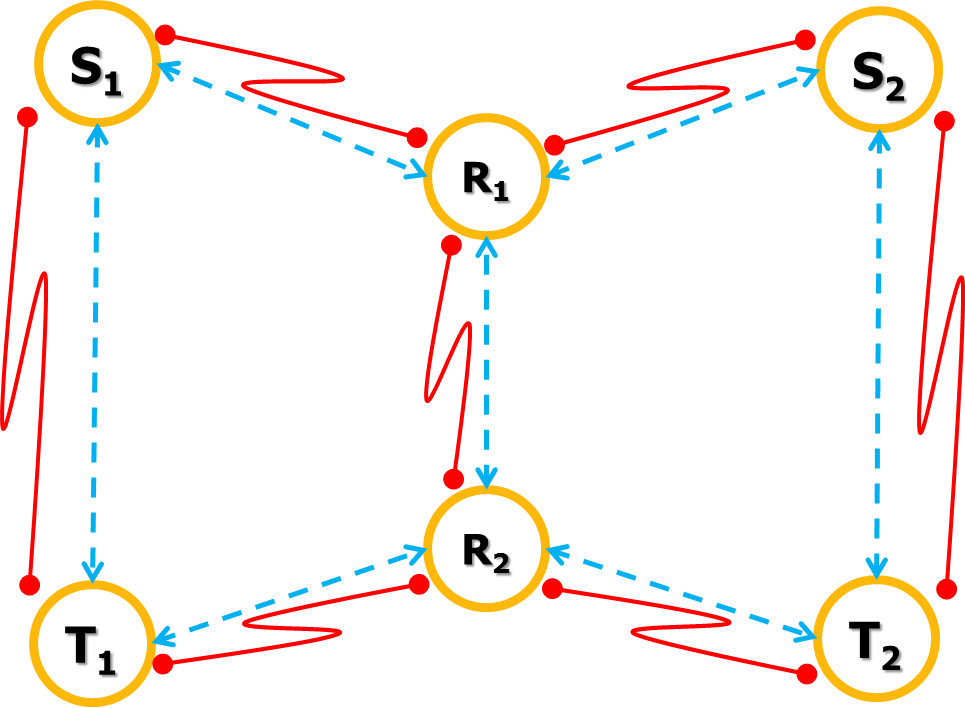
\includegraphics[width=0.35\textwidth]{butterflyquantum.png}
      \end{center}
      \vspace{-15pt}
    \end{wrapfigure}
    Una red troncal simétrica, conocida también como \textbf{``Red mariposa''}, es una red compuesta por una cantidad par de parejas de usuarios fuente-objetivo, que se encuentran conectados entre sí y a su vez a un enlace troncal de repetidores. Las redes mariposa a considerar se diferencian por la cantidad de pares de usuarios $M$ y la cantidad $N$ de enlaces entre las repetidoras de la ruta troncal. \par
    En este tipo de redes, sobre los diferentes nodos de la red se aplican las operaciones de codificación ya descritas en función de $M$ y $N$.
  \end{block}
\end{frame}

%%------------------------------------%%
\begin{frame}{Codificación de una red cuántica para una red troncal simétrica}
  \begin{block}{Red mariposa N=1, M=2}
    La red mariposa más simple es aquella con $N=1$ saltos entre repetidoras y $M=2$ pares de usuarios.
    \begin{figure}
      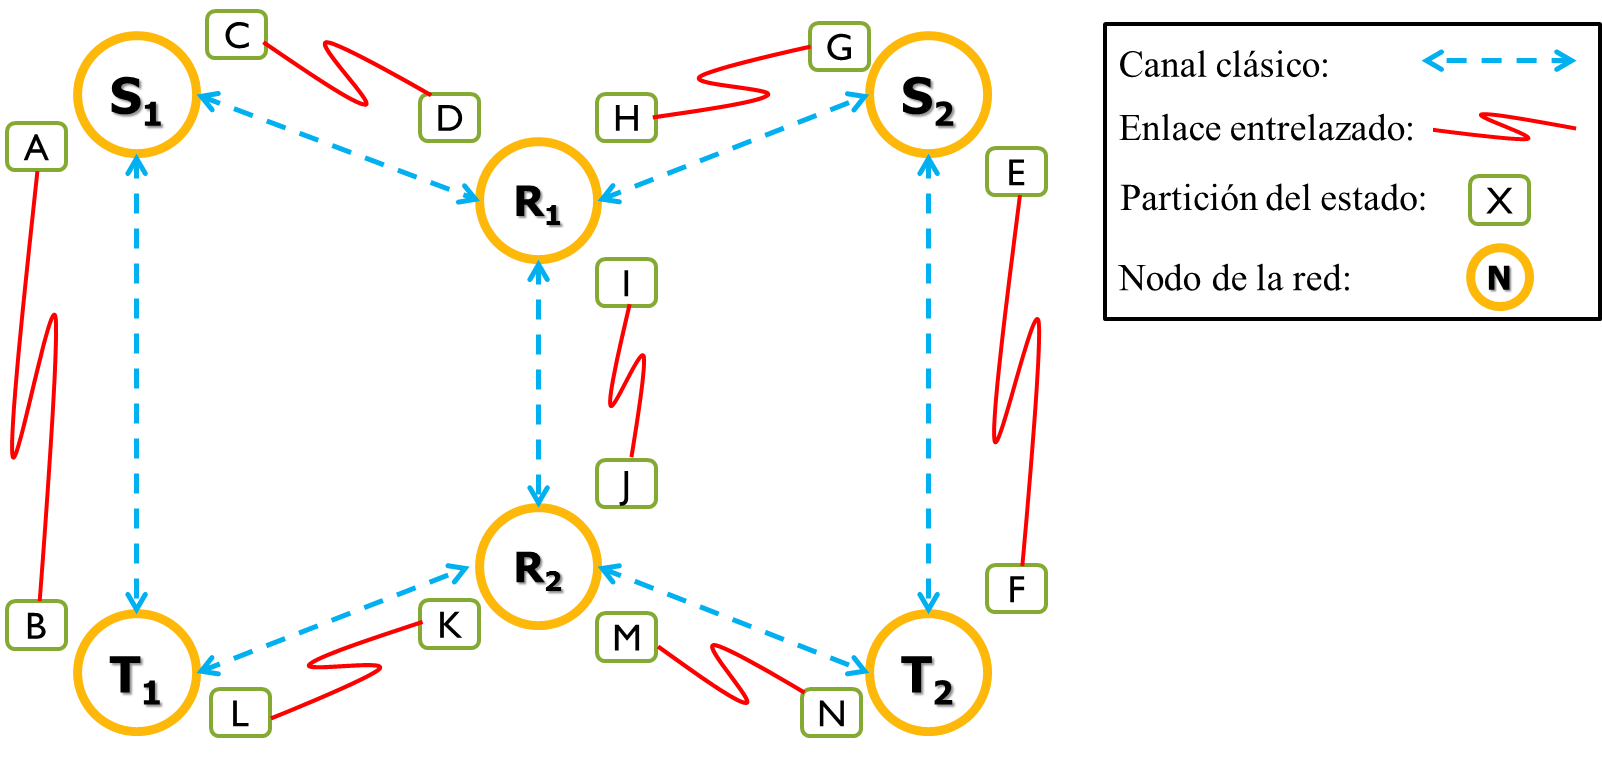
\includegraphics[width=0.8\textwidth]{butterflyquantum2.png}
      \caption{Red cuántica tipo mariposa, luego de distribuir entrelazamiento y antes de la codificación.}
      \label{fig:butterfly2}
    \end{figure}%
  \end{block}

\end{frame}


%%------------------------------------%%
\begin{frame}{Codificación de una red cuántica para una red troncal simétrica}

  \begin{table}
    \caption{Etapas de la codificación de la red tipo mariposa para el caso $N=1$ y $M=2$}
    \begin{tabular}{|c|l|l|}
      \hline
      Fases & \multicolumn{1}{c|}{Operaciones}             & \multicolumn{1}{c|}{Nodos}  \\ \hline
      1     & $Con^A_{C \rightarrow D}$                    & $S_1  \rightarrow R_1$      \\
            & $Con^E_{G  \rightarrow H}$                   & $S_2  \rightarrow R_1$      \\ \hline
      2     & $Add^{D,H}_{I  \rightarrow J}$               & $R_1  \rightarrow R_2$      \\ \hline
      3     & $Fan^J_{K  \rightarrow L, M  \rightarrow N}$ & $R_2  \rightarrow T_1, T_2$ \\ \hline
      4     & $CNOT_{L,B}$                                 & $T_1$                       \\
            & $CNOT_{N,F}$                                 & $T_2$                       \\ \hline
      5     & $Rem_{L  \rightarrow J}$                     & $T_1  \rightarrow R_2$      \\
            & $Rem_{N  \rightarrow J}$                     & $T_2  \rightarrow R_2$      \\ \hline
      6     & $RemAdd_{J  \rightarrow D,H}$                & $R_2  \rightarrow R_1$      \\ \hline
      7     & $Rem_{D  \rightarrow A}$                     & $R_1  \rightarrow S_1$      \\
            & $Rem_{H  \rightarrow E}$                     & $R_1  \rightarrow S_2$      \\ \hline
    \end{tabular}
    \vspace{-0.5cm}
  \end{table}

\end{frame}
%%------------------------------------%%
\begin{frame}{Cálculos de la codificación de redes cuánticas simétricas}
  Por tratarse de operaciones no unitarias los estados al final de la codificación no se encuentran normalizados, sin embargo conociendo que estos estados finales serán máximamente entrelazados se entiende que al normalizar se obtiene que la amplitud de probabilidad de cada par EPR es de $\dfrac{1}{\sqrt{2}}$.
  \begin{block}{Red mariposa N=1, M=2}
    Se muestran los cálculos de la codificación de la red tipo mariposa más simple, donde $M=2$ representan dos pares de usuarios emisor y receptor, y $N=1$ representa la cantidad de saltos entre las repetidoras de la línea troncal. \par
    Siguiendo la Figura \ref{fig:butterfly2} al inicio se tienen siete estados entrelazados entre cada vértice de la red que corresponden al siguiente estado inicial.
    \begin{align*}
      \ket{\psi_{inicial}} = \ket{MN}\ket{KL}\ket{IJ}\ket{GH}\ket{EF}\ket{CD}\ket{AB}
    \end{align*}
  \end{block}
\end{frame}

\begin{frame}{Cálculos para una red mariposa N=1, M=2}
  \textbf{Fase 1:} Se aplican las operaciones $Con^{A}_{C \rightarrow D}$, y $Con^{E}_{G \rightarrow H}$. Esto resulta en:
  \begin{align*}
  \ket{\psi_{1}} = \ket{MN} \ket{KL} \ket{IJ} 
  [\frac{1}{\sqrt{2}} (\ket{000}_{EFH} + \ket{111}_{EFH})] 
  [\frac{1}{\sqrt{2}} (\ket{000}_{ABD} + \ket{111}_{ABD})] 
  \end{align*}
  \textbf{Fase 2:} Se aplica $ Add^{D,H}_{I \rightarrow J} $. Reescribimos $\ket{\psi_{1}}$
\begin{align*}
\ket{\psi_{1}}=\ket{MN}\ket{KL}\ket{IJ} ( 
& \ket{000}_{EFH}\ket{000}_{ABD} + \ket{000}_{EFH}\ket{111}_{ABD} + \\
& \ket{111}_{EFH}\ket{000}_{ABD} + \ket{111}_{EFH}\ket{111}_{ABD} + 
\end{align*}
Se aplica la operación.
\begin{align*}
\ket{\psi_{2}} =& Add^{D,H}_{I \rightarrow J}  \ket{\psi_{1}} \\
\ket{\psi_{2}} =& 
\ket{MN} \ket{KL} \ket{000}_{EFH}\ket{000}_{ABD}\ket{0}_J +\ket{MN}\ket{KL}\ket{000}_{EFH}\ket{111}_{ABD} \ket{1}_J \\
+& \ket{MN} \ket{KL} \ket{111}_{EFH}\ket{000}_{ABD}\ket{1}_J +\ket{MN}\ket{KL}\ket{111}_{EFH}\ket{111}_{ABD} \ket{0}_J
\end{align*}
\alert{Hasta ahora, se han descartado las particiones ``C'', ``G'', y ``I''.}
\end{frame}

\begin{frame}{Cálculos para una red mariposa N=1, M=2}
  \textbf{Fase 3:} Se aplica la operación $Fan^{J}_{K\rightarrow L, M\rightarrow N}$. Recordando que las operaciones de codificación están compuestas de operaciones unitarias y medidas, separamos esta operación ``Fan'' en partes. \par
  El circuito cuántico para esta Fase 3 sería el siguiente:
  \begin{figure}
    \[
      \Qcircuit @C=2em @R=0em @!R{
      \lstick{\ket{J}} & \ctrl{2} & \ctrl{5} & \qw & \qw & \qw \\
      &  & & & \\
      \lstick{\ket{K}} & \targ &  \qw & \measure{M_Z} & \cctrl{1} & \\
      \lstick{\ket{L}} & \qw & \qw &  \qw &\gate{X} & \qw \\
      &  & & & \\
      \lstick{\ket{M}} & \qw &  \targ & \measure{M_Z} & \cctrl{1} & \\
      \lstick{\ket{N}} & \qw & \qw &  \qw & \gate{X} & \qw \\
      }\]
    \caption{Diagrama de circuito cuántico de la Fase 3}
  \end{figure}
\end{frame}
% --------------------------
\begin{frame}{Cálculos para una red mariposa N=1, M=2}
  \begin{alertblock}{Fase 3: Parte a.}
    Esta parte se refiere a la operación $CNOT^J_{K,M}$ al inicio del circuito, el estado resultante queda así.
    \begin{align*}
      \ket{\psi_{3.a}} = & \qty[\frac{1}{2}(\ket{00}_{MN}+\ket{11}_{MN})(\ket{00}_{KL}+\ket{11}_{KL})]\ket{000}_{EFH}\ket{000}_{ABD}\ket{0}_{J} \\
      + & \qty[\frac{1}{2}(\ket{10}_{MN}+\ket{01}_{MN})(\ket{10}_{KL}+\ket{01}_{KL})]\ket{000}_{EFH}\ket{111}_{ABD}\ket{1}_{J} \\
      + & \qty[\frac{1}{2}(\ket{10}_{MN}+\ket{01}_{MN})(\ket{10}_{KL}+\ket{01}_{KL})]\ket{111}_{EFH}\ket{000}_{ABD}\ket{1}_{J} \\
      + & \qty[\frac{1}{2}(\ket{00}_{MN}+\ket{11}_{MN})(\ket{00}_{KL}+\ket{11}_{KL})]\ket{111}_{EFH}\ket{111}_{ABD}\ket{0}_{J} 
    \end{align*}
  \end{alertblock}
\end{frame}
% ------------------------
\begin{frame}{Cálculos para una red mariposa N=1, M=2}
  \begin{alertblock}{Fase 3: Parte b.}
    Esta parte se refiere a la medida en ``M'', eliminar el registro y controlar la compuerta $X$.
    \begin{align*}
    \ket{\psi_{3.b}} = & \qty[ \frac{1}{\sqrt{2}} \ket{0}_{N}(\ket{00}_{KL}+\ket{11}_{KL})]\ket{000}_{EFH}\ket{000}_{ABD}\ket{0}_{J} \\
                      + & \qty[ \frac{1}{\sqrt{2}} \ket{1}_{N}(\ket{10}_{KL}+\ket{01}_{KL})]\ket{000}_{EFH}\ket{111}_{ABD}\ket{1}_{J}
    \end{align*}
  \end{alertblock}
  \begin{alertblock}{Fase 3: Parte c.}
    Esta parte se refiere a la medida en ``K'', eliminar el registro y controlar la compuerta $X$.
    \begin{align*}
    \ket{\psi_{3.c}}
    = & \ket{0}_{N} \ket{0}_{L} \ket{000}_{EFH} \ket{000}_{ABD} \ket{0}_{J}
      + \ket{1}_{N} \ket{1}_{L} \ket{000}_{EFH} \ket{111}_{ABD} \ket{1}_{J} \\
    + & \ket{1}_{N} \ket{1}_{L} \ket{111}_{EFH} \ket{000}_{ABD} \ket{1}_{J} 
      + \ket{0}_{N} \ket{0}_{L} \ket{111}_{EFH} \ket{111}_{ABD} \ket{0}_{J} 
    \end{align*}
  \end{alertblock}
\end{frame}

\begin{frame}{Cálculos para una red mariposa N=1, M=2}
  \begin{alertblock}{Fase 3: Resultado}
    Reescribiendo, al finalizar la Fase 3:
    \begin{align*}
    \ket{\psi_{3}}=&\ket{000}_{EFH} \ket{000}_{ABD} \ket{000}_{JNL} +\ket{000}_{EFH} \ket{111}_{ABD} \ket{111}_{JNL} \\
    +&\ket{111}_{EFH} \ket{000}_{ABD} \ket{111}_{JNL} + \ket{111}_{EFH} \ket{111}_{ABD} \ket{000}_{JNL} 
    \end{align*}
  \end{alertblock}
\end{frame}

\begin{frame}{Cálculos para una red mariposa N=1, M=2}
  \textbf{Fase 4:} Operaciones $ CNOT_{L,B} $ y $ CNOT_{N,F} $.
    \begin{align*}
    \ket{\psi_{4}} = 
      & \ket{000}_{EFH} \ket{000}_{ABD} \ket{000}_{JNL} + \ket{010}_{EFH} \ket{101}_{ABD} \ket{111}_{JNL} \\
    +& \ket{101}_{EFH} \ket{010}_{ABD} \ket{111}_{JNL} + \ket{111}_{EFH} \ket{111}_{ABD} \ket{000}_{JNL}  
    \end{align*}
  \textbf{Fase 5:} Operaciones $ Rem_{L \rightarrow J} $ y  $ Rem_{N \rightarrow J} $ 
  \begin{align*}
  \ket{\psi_5}=  Rem_{L \rightarrow J} \ket{\psi_4} = Rem_{L \rightarrow J} & [ \ket{000}_{JNL}(\ket{000}_{EFH} \ket{000}_{ABD}+\ket{111}_{EFH} \ket{111}_{ABD}) \\
  + & \ket{111}_{JNL}(\ket{010}_{EFH} \ket{101}_{ABD}+\ket{101}_{EFH} \ket{010}_{ABD})]
  \end{align*}
  Hadamard en ``L'':
  \begin{align*}
  \ket{\psi_{5.a}}= & \dfrac{1}{\sqrt{2}}  (\ket{000}_{JNL}+\ket{001}_{JNL})(\ket{000}_{EFH}\ket{000}_{ABD}+\ket{111}_{EFH}\ket{111}_{ABD}) \\
  + & \dfrac{1}{\sqrt{2}} (\ket{110}_{JNL}-\ket{111}_{JNL})(\ket{010}_{EFH} \ket{101}_{ABD}+\ket{101}_{EFH} \ket{010}_{ABD})
  \end{align*}
\end{frame}

\begin{frame}{Cálculos para una red mariposa N=1, M=2}
  Medir en ``L'' y controlar $Z$ en ``J'' y descartar ``L'':
  \begin{align*}
  \ket{\psi_{5.b}} & = \ket{00}_{JN}(\ket{000}_{EFH}\ket{000}_{ABD}+\ket{111}_{EFH} \ket{111}_{ABD}) \\
  & + \ket{11}_{JN}(\ket{010}_{EFH}\ket{101}_{ABD}+\ket{101}_{EFH} \ket{010}_{ABD})
  \end{align*}
  Ahora se realiza el segundo Removal. Hadamard en ``N'':
  \begin{align*}
  \ket{\psi_{5.c}} &= \dfrac{1}{\sqrt{2}} (\ket{00}_{JN}+\ket{01}_{JN})(\ket{000}_{EFH}\ket{000}_{ABD}+\ket{111}_{EFH} \ket{111}_{ABD}) \\
  &+ \dfrac{1}{\sqrt{2}} (\ket{10}_{JN}-\ket{11}_{JN})(\ket{010}_{EFH}\ket{101}_{ABD}+\ket{101}_{EFH} \ket{010}_{ABD})
  \end{align*}
  Medir en ``N'' y controlar compuerta $Z$, se descarta ``N''.
  \begin{align*}
  \ket{\psi_5} = & \ket{0}_{J}(\ket{000000}_{EFHABD}+\ket{111111}_{EFHABD}) \\
  + & \ket{1}_{J}(\ket{010101}_{EFHABD}+\ket{101010}_{EFHABD})
  \end{align*}
\end{frame}

\begin{frame}{Cálculos para una red mariposa N=1, M=2}
  \textbf{Fase 6:} Operación $RemAdd_{J \rightarrow D,H}$, se realiza un Hadamard en ``J'' se mide y se controlan las compuertas $Z$ en ``D'' y ``H'', resulta en:
  \begin{align*}
  \ket{\psi_6} = \ket{000000}_{EFHABD}+\ket{010101}_{EFHABD}+\ket{101010}_{EFHABD}+\ket{111111}_{EFHABD} 
  \end{align*}
  \textbf{Fase 7:} Operación  $ Rem_{D \rightarrow A} $ y  $ Rem_{H \rightarrow E} $, esto queda en:
  \begin{align*}
  \ket{\psi_7} = \ket{00}_{EF} \ket{00}_{AB} + \ket{01}_{EF} \ket{10}_{AB} + \ket{10}_{EF} \ket{01}_{AB} + \ket{11}_{EF} \ket{11}_{AB} 
  \end{align*}
\end{frame}

\begin{frame}{Cálculos para una red mariposa N=1, M=2}
  Esta última fue la operación final, reescribiendo tenemos:
  \begin{align*}
  \ket{\psi_{f}} =\ket{0}_{A} \ket{0}_{F} \ket{0}_{B}\ket{0}_{E} + \ket{1}_{A}
                  \ket{1}_{F}\ket{0}_{B}\ket{0}_{E} \\ 
                  +\ket{0}_{A} \ket{0}_{F} \ket{1}_{B}\ket{1}_{E} + \ket{1}_{A}
                  \ket{1}_{F}\ket{1}_{b}\ket{1}_{E}
  \end{align*}
  Factorizando
  \begin{align*}
  \ket{\psi_{f}} = \ket{00}_{AF}  (\ket{00}_{BE}+\ket{11}_{BE}) + \ket{11}_{AF}(\ket{00}_{BE}+\ket{11}_{BE})
  \end{align*}
  Se obtiene como estado final:
  \begin{align*}
  \ket{\psi_f} = (\ket{00}_{AF}+\ket{11}_{AF})(\ket{00}_{BE}+\ket{11}_{BE})
  \end{align*}
\end{frame}
%%------------------------------------%%
\begin{frame}{Codificación de una red cuántica para una red troncal simétrica}
  \begin{block}{}
    Luego de las operaciones de codificación, se tiene el entrelazamiento requerido.
    \begin{figure}
      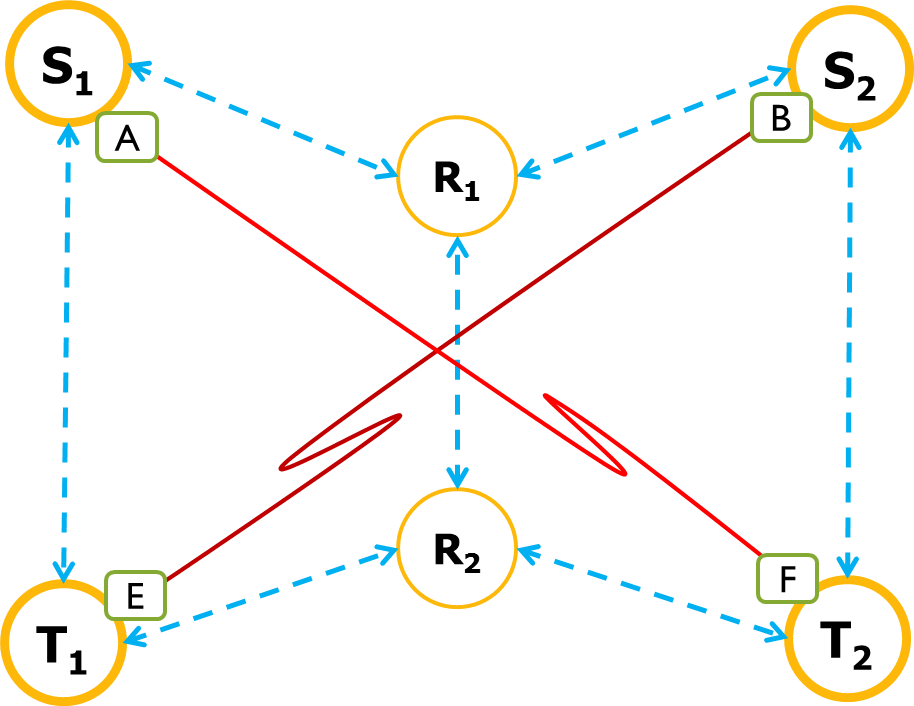
\includegraphics[width=0.6\textwidth]{butterflycoded2.png}
      \caption{Red cuántica luego de la codificación}
    \end{figure}
  \end{block}
\end{frame}

%%------------------------------------%%
\begin{frame}{Codificación de una red cuántica para una red troncal simétrica}

  \begin{block}{}
    \vspace{-3cm}
    \begin{wrapfigure}{r}{0.45\textwidth}
      \vspace{-15pt}
      \begin{center}
        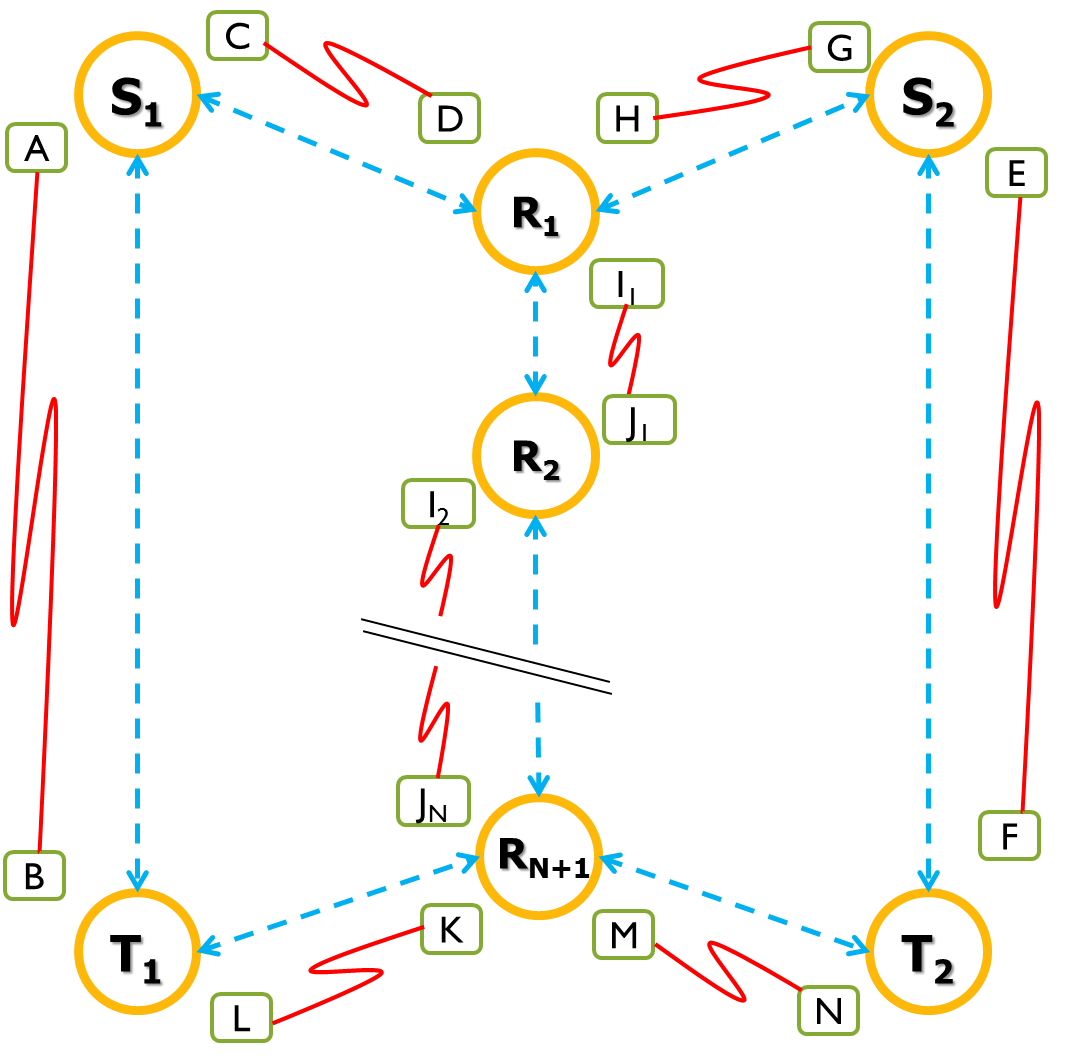
\includegraphics[width=0.4\textwidth]{butterflynnnm22.png}
      \end{center}
      \vspace{-15pt}
      \caption{Red mariposa con N saltos arbitrarios y M=2 pares de usuarios}
    \end{wrapfigure}
    Existen otros tipos de redes mariposa de mayor tamaño, al aumentar la cantidad de saltos $N$ entre repetidores es necesario añadir una Fase de codificación que enlace todo el troncal, al aumentar la cantidad de usuarios $M$ aumentan las operaciones dentro de cada Fase.
  \end{block}
\end{frame}

%%------------------------------------%%
\begin{frame}{Codificación de una red cuántica para una red troncal simétrica}
  \begin{block}{}
    \begin{figure}
      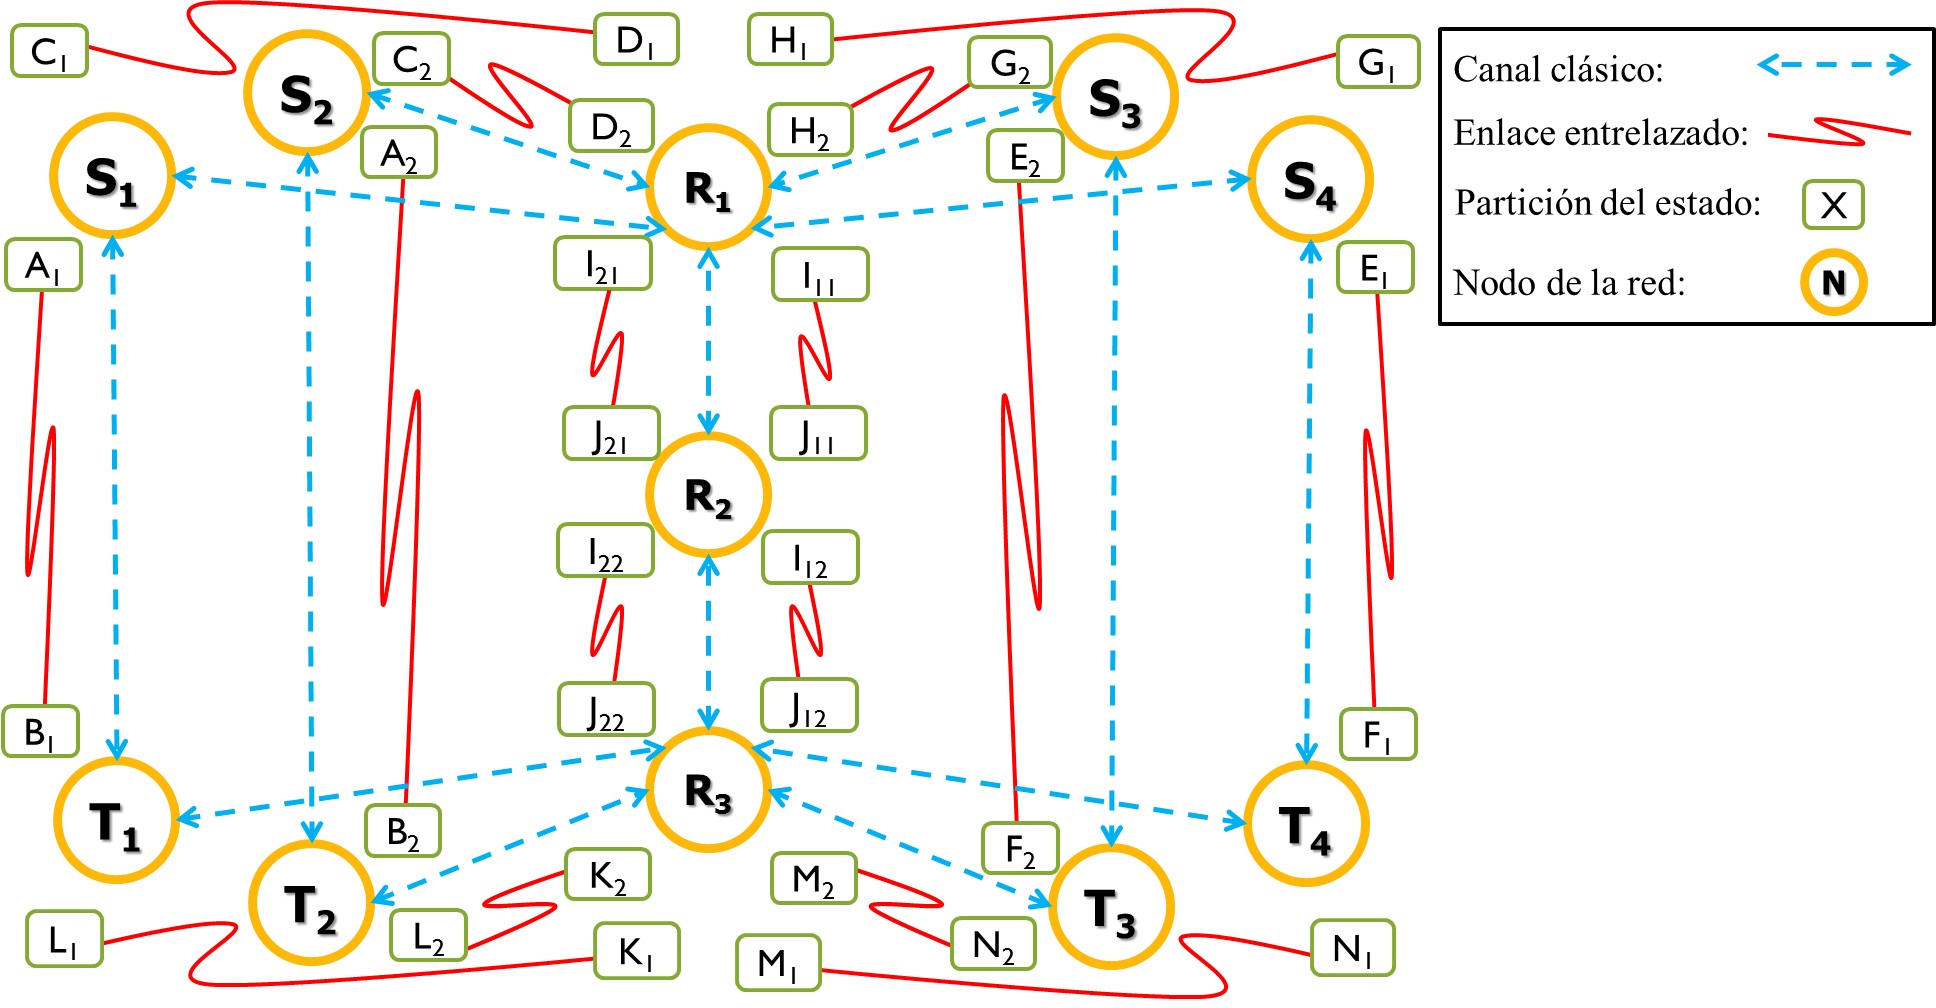
\includegraphics[width=0.8\textwidth]{butterflyn2m4.png}
      \caption{Red cuántica tipo mariposa para el caso N=2 y M=4}
    \end{figure}
  \end{block}
\end{frame}


%%------------------------------------%%
\begin{frame}{Codificación de una red cuántica para una red troncal simétrica}
  \begin{block}{}
    \vspace{-20pt}
    \begin{figure}
      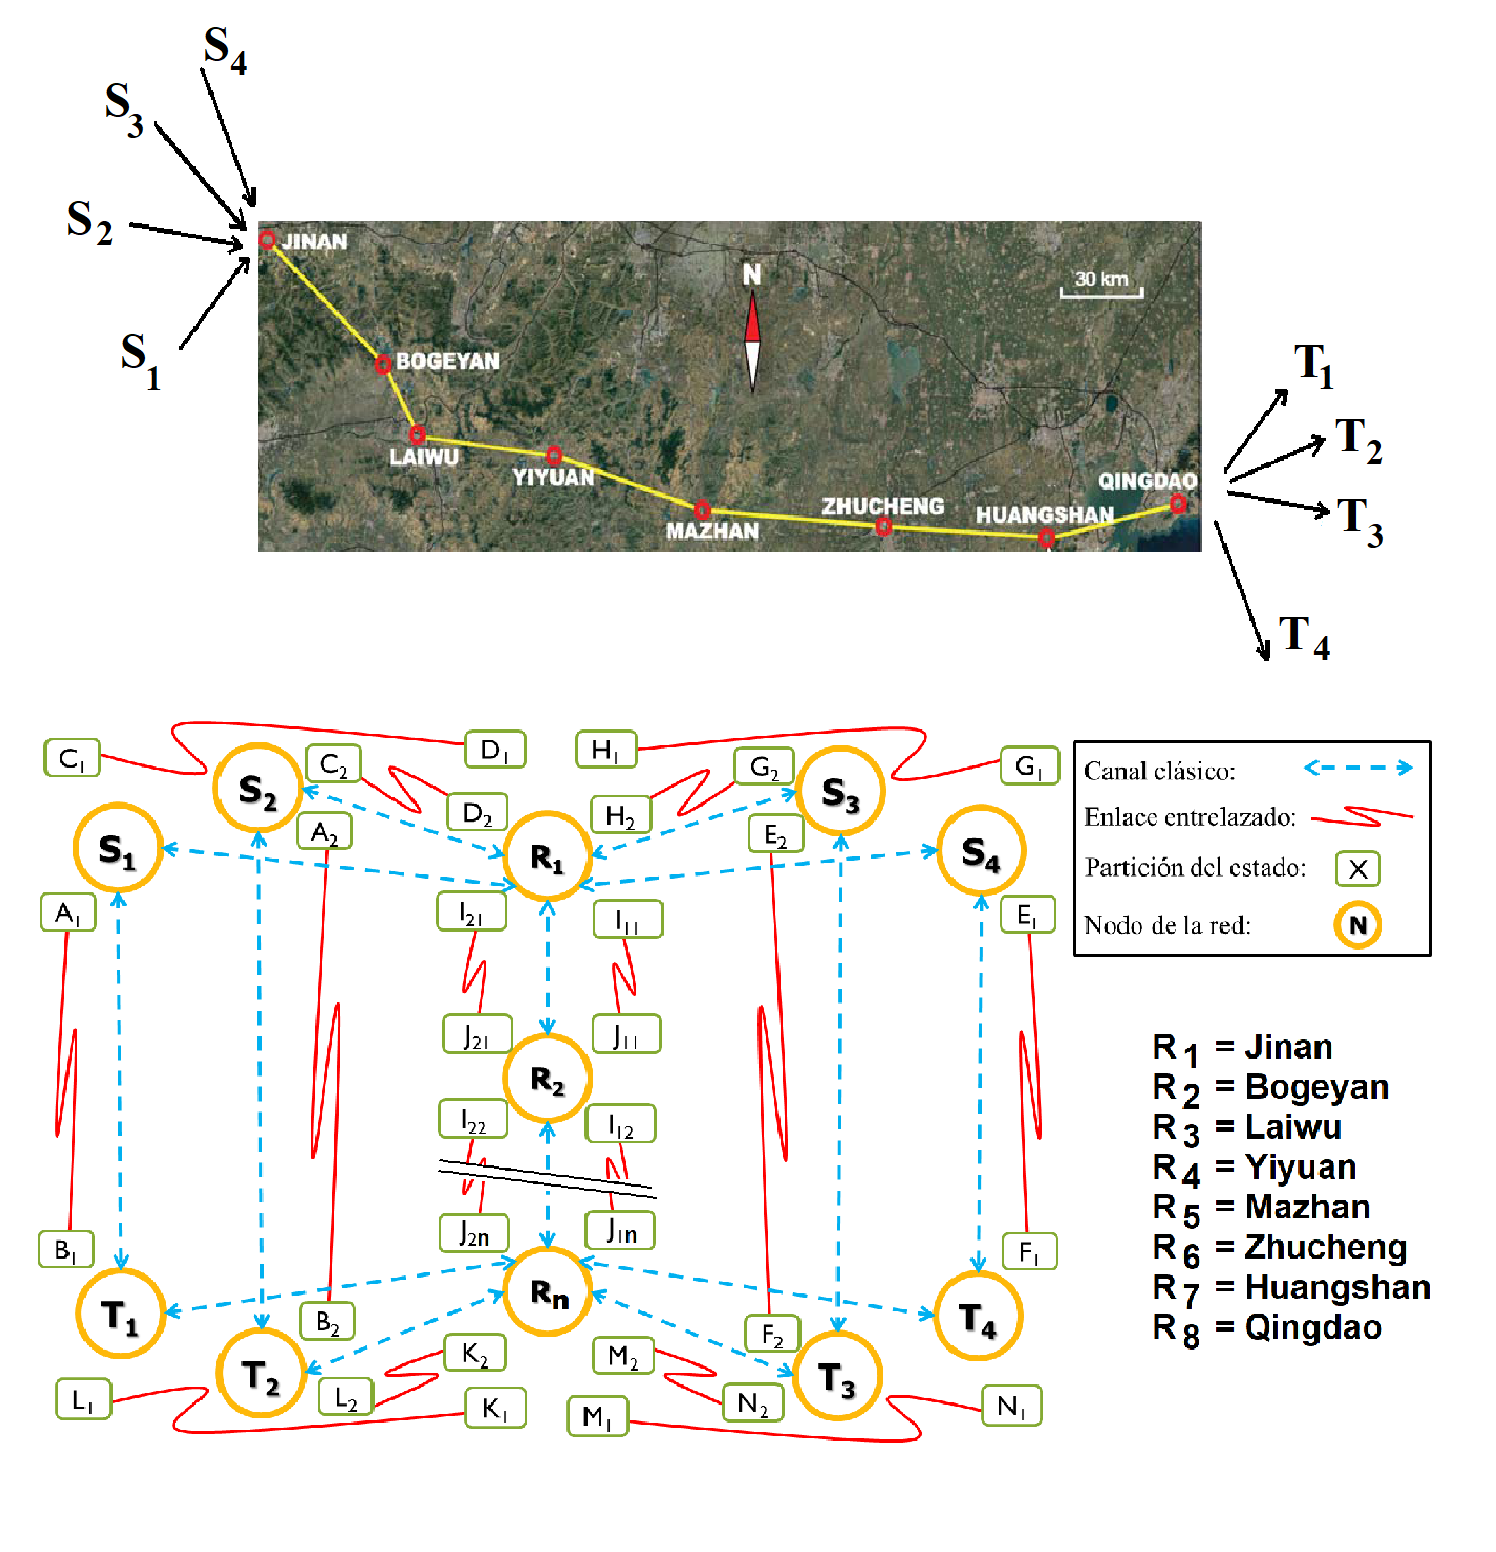
\includegraphics[width=0.7\textwidth]{Hguyenchina.png}
      \caption{Red troncal de china que se puede adaptar y codificar mediante este método.}
    \end{figure}
  \end{block}
\end{frame}
%%------------------------------------%%
\begin{frame}{Distribución de entrelazamiento}
  \begin{block}{Distribución o intercambio de entrelazamiento}
    Dado que se desea como objetivo realizar teleportación, y la teleportación requiere entrelazamiento a distancia, principalmente las redes cuánticas requieren distribuir entrelazamiento entre los nodos cercanos conectados por canales cuánticos. \par
    La distribución de entrelazamiento se basa principalmente en la generación de entrelazamiento con fotones que son enviados por canales de fibra óptica o espacio libre hacia dos nodos adyacentes, estableciendo entrelazamiento a distancia. \par
    Posterior a la distribución de entrelazamiento entre nodos cercanos, se necesita lograr un entrelazamiento a mayor escala, esto se puede lograr mediante la \alert{codificación} de la red.
  \end{block}
\end{frame}

\begin{frame}{Intercambio de Entrelazamiento}
  \begin{block}{}
    Este protocolo de codificación de red busca establecer el entrelazamiento entre dos qubits lejanos, consiste en conectar dos pares entrelazados para obtener uno solo a una distancia mayor, esto se logra posterior a la distribución de entrelazamiento entre repetidoras cercanas. Este método es el más sencillo e intuitivo para conectar un par fuente-objetivo que se encuentra separados por una o más repetidoras cuánticas.
  \end{block}
  \begin{block}{Se utilizan las operaciones siguientes en este orden}
    \begin{enumerate}
      \item La operación \textit{Connect}, $Con^B_{C -> D}$, que conecta \K{B} con \K{C}, mide \K{C} y envía información clásica a \K{D}, la partición \K{C} será descartada.
      \item La operación \textit{Removal}, $Rem_{B -> A}$, que mide en \K{B} y envía información clásica a \K{A}, la partición \K{B} será descartada.
    \end{enumerate}

  \end{block}
\end{frame}
%%------------------------------------%%
\begin{frame}{Intercambio de Entrelazamiento}
  \begin{block}{}
    \begin{figure}
      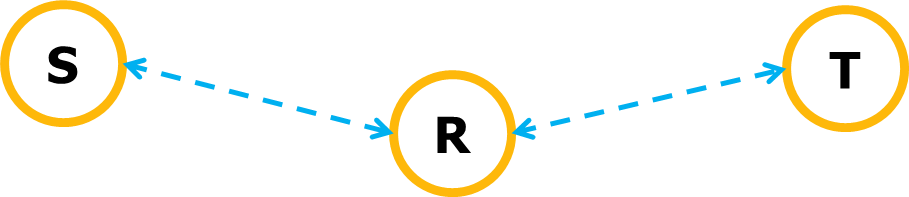
\includegraphics[width=0.6\textwidth]{Imagen1.png}
      \caption{Esquema de tres nodos.}
    \end{figure}
  \end{block}
\end{frame}
\begin{frame}{Intercambio de Entrelazamiento}
  \begin{block}{}
    \begin{figure}
      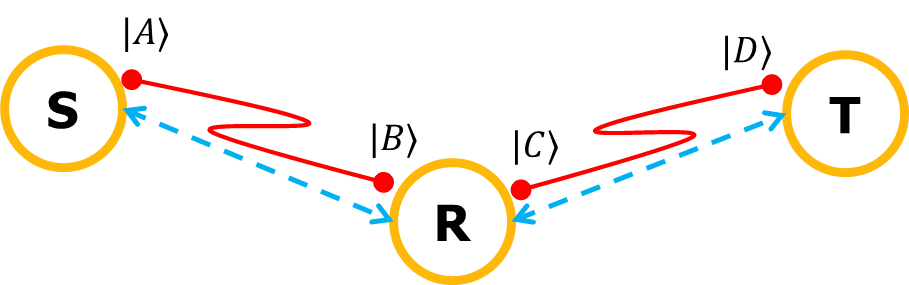
\includegraphics[width=0.6\textwidth]{Imagen2.png}
      \caption{Esquema de tres nodos, luego de distribuir el entrelazamiento.}
    \end{figure}
  \end{block}
\end{frame}
\begin{frame}{Intercambio de Entrelazamiento}
  \begin{block}{}
    \begin{figure}
      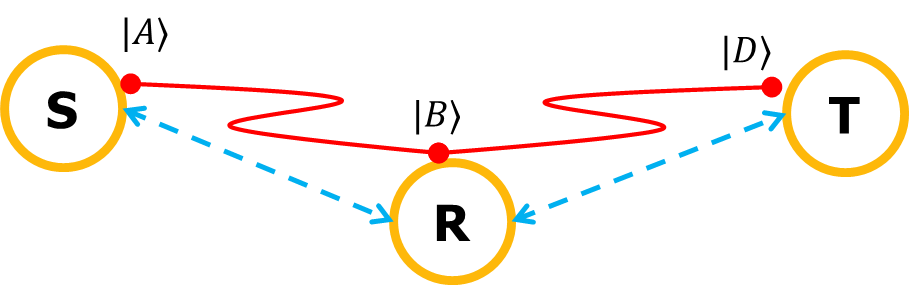
\includegraphics[width=0.6\textwidth]{Imagen3.png}
      \caption{Esquema de tres nodos, luego de aplicar Connect en el repetidor.}
    \end{figure}
  \end{block}
\end{frame}
\begin{frame}{Intercambio de Entrelazamiento}
  \begin{block}{}
    \begin{figure}
      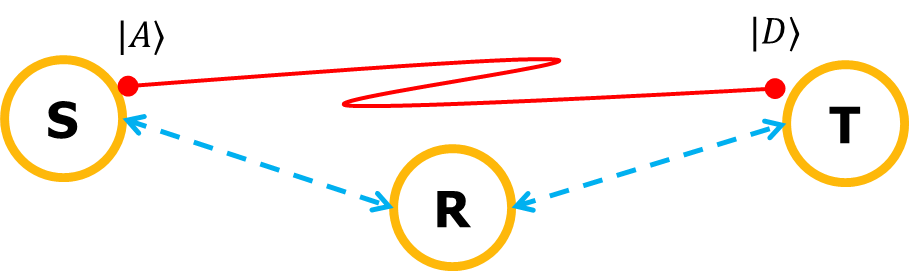
\includegraphics[width=0.6\textwidth]{Imagen4.png}
      \caption{Esquema de tres nodos, luego de aplicar Removal en el repetidor. Se obtiene entonces el entrelazamiento requerido para aplicar la teleportación.}
    \end{figure}
  \end{block}
\end{frame}
%%-----------------
%%------------------------------------%%
\section{Esquema general de la red de comunicación cuántica}
\begin{frame}{Esquema general de la red cuántica}
  \begin{block}{Capa física clásica y cuántica}
    La red cuántica y sus capas requieren de un canal clásico auxiliar para comunicar información sobre las medidas y operaciones realizadas. Y la capa física cuántica se compone del medio o canal por el cual se transmiten los estados cuánticos como fotones, este canal puede ser espacio libre (aire), o bien fibras ópticas. Para este esquema, en esta capa los estados que se transmiten son estados entrelazados EPR.
  \end{block}
  \begin{block}{Capa de entrelazamiento}
    Es necesario distribuir el entrelazamiento entre los nodos adyacentes de la red. La codificación de las redes requiere que los nodos compartan pares entrelazados inicialmente.
  \end{block}
\end{frame}
%%------------------------------------%%
\begin{frame}{Esquema general de la red cuántica}

  \begin{block}{Capa de codificación de red}
    Para lograr el entrelazamiento entre nodos distantes más allá de los nodos adyacentes, existen diversos métodos de codificación que varían dependiendo de la topología, el entrelazamiento a distancia es un recurso fundamental de la teleportación de la capa superior y es la contribución principal del paper de Nguyen.
  \end{block}
  \begin{block}{Capa de teleportación}
    Luego de tener el entrelazamiento deseado se puede teleportar información cuántica, o bien utilizar el entrelazamiento para otro propósito.
  \end{block}
  \begin{block}{Capa de seguridad}
    Sobre la teleportación pueden realizarze protocolos de criptografía cuántica, por ejemplo se pueden usar protocolos QKD que consisten en distribuir claves cuánticas.
  \end{block}

\end{frame}

%%%%%%%%%%%%%%%%%%%%%%%%%%%%%%%%%%%%%%%%%%%%%%%%
\section{Conclusiones}

\begin{frame}{Conclusiones}
  Para resumir, el diseño de LQNC puede ser llevado a cabo usando los siguientes pasos.
  \begin{enumerate}
    \setcounter{enumi}{0}
    \item Se requiere partir la red compleja dada en fragmentos. Entonces el más beneficioso entre los protocolos ES y LQNC puede ser usado para convertir la estructura arbitraria de los fragmentos a una extensión de la red mariposa.
    
    \item Luego se interpretan los detalles de los requerimientos de diseño. Que puede abarcar los parámetros característicos de un sistema LQNC, incluyendo el número involucrado de pares M entrelazados y la fidelidad a la entrada y la salida, así como el número de repetidoras cuánticas disponibles definiendo el número de saltos N. Esto se puede notar que se debe a la conversión del paso 1, la fidelidad de un particular par entrelazado de qubits puede variar a través de la red, por lo tanto las distintas probabilidades de error se vuelven utiles.

  \end{enumerate}
\end{frame}

\begin{frame}{Conclusiones}
  \begin{enumerate}
    \setcounter{enumi}{2}
    \item Posteriormente Nguyen construye la arquitectura general del sistema y se determina su configuración basándose en las limitaciones y las especificaciones dadas. Luego, procede mediante la construcción del proceso específico de codificación y decodificación, lo cual conduce a patrones de error específico que pueden ser usados para predecir el desempeño del sistema.
  \end{enumerate}
\end{frame}

  \begin{frame} 
    \begin{alertblock}{Conclusión}
      El paper de Nguyen muestra los beneficios de la codificación De redes cuánticas en el contexto de redes cuánticas a gran escala, Los sistemas basados en LQNC  son capaces de proveer 10 veces mejor rendimiento infidelidad a una alta tasa de codificación mayor que Los sistemas basados en ES cuando se considera una red a gran escala.
    \end{alertblock}
  \end{frame}

%%%%%%%%%%%%%%%%%%%%%%%%%%%%%%%%%%%%%%%%%%%%%%%%
\begin{frame}[standout]
  Muchas Gracias.
\end{frame}


{\setbeamercolor{palette primary}{fg=black, bg=yellow}
\begin{frame}[standout]
  Preguntas.
\end{frame}
}
% %%%%%%%%%%%%%%%%%%%%%%%%%%%%%%%%%%%%%%%%%%%%%%%%%%%%%%%%%%

\end{document}
